\textbf{Chapter 9 Quadratic Residues}
\[ Q_n = \set{x^2}{x\in U_n} \]
Problem: given $a\in U_n$ determine whether $a\in Q_n$

for $\gcd(k,l)=1$
\begin{align*}
U_{kl} &\cong U_k \oplus U_l \\
Q_{kl} &\cong U_k \oplus Q_l
\end{align*}
It suffices to consider $U_{p^k}$ for $p$ prime.

$U_2=\brace1$, $Q_2=\brace1$ \\
$U_4=\brace{1,3}$, $Q_4=\brace1$ \\
$U_{2^k}=\brace{\pm5^i}$, $Q_{2^k}=\brace{+5^{2i}}$, $\abs{Q_{2^k}}=\frac14\abs{U_{2^k}}=\frac14\phi(2^k)=2^{k-3}$ \\
$U_{p^k}=\chev{u}=\brace{u^i}$, $Q_{p^k}=\chev{u^2}=\brace{u^{2i}}$, $\abs{Q_{p^k}}=\frac12\abs{U_{p^k}}=\frac12\phi(p^k)=\frac12p^{k-1}(p-1)$

\eg For $a\in U_{2^k}$ with $k\geq3$ we have $a\in Q_{2^k}\iff a=1\bmod8$
\[ U_{2^k} = \chev{\pm5^i} = \brace{5^0,5^2,5^4,\dotsc}\footnote{$=Q_{2^k}=\set{a\in U_{2^k}}{a=1\bmod8}$} \cup \brace{5^1,5^3,5^5,\dotsc}\footnote{$5\bmod8$} \cup \brace{-5^0,-5^2,\dotsc}\footnote{$7\bmod8$} \cup \brace{-5^1,-5^3,\dotsc}\footnote{$3\bmod8$} \]
\note For an odd prime $p$,
\[ a\in Q_{p^k} \iff a\in Q_p \]
\pf Say $U_{p^k}=\chev{u}$.  Then $U_p=\chev{u}$.
\begin{align*}
a\in Q_{p^k} &\iff \text{$a=u^k$ for some even $k$} \\
&\iff a\in U_p
\end{align*}
Our problem is reduced to the following: \\
given $a\in U_p$ where $p$ is an odd prime, determine whether $a\in Q_p$

\defn For an odd prime $p$ and for $a\in\Z$, we define the \emph{Legendre symbol}
\[ \leg{a}{p} = (a|p) = \begin{cases}
0 & \text{if $a\notin U_p$ (i.e., $p\div a$)} \\
1 & \text{if $a\in Q_p$} \\
-1 & \text{if $a\in U_p\setminus Q_p$}
\end{cases} \]
\note For $a\in U_p=\chev{u}$ with say $a=u^k$, $a\in Q_p\iff\text{$k$ is even}$ so
\[ \leg{a}{p} = (-1)^k \]
\thm Let $p$ be an odd prime and let $a$, $b\in\Z$.  Then
\[ \leg{ab}{p} = \leg{a}{p}\leg{b}{p} \]
\pf if $p\div a$ or $p\div b$ (so $a\notin U_p$ or $b\notin U_p$) then $p\div ab$ so
\[ \leg{ab}{p} = 0 = \leg{a}{p} \leg{b}{p} \]
If $a$, $b\in U_p=\chev{u}$ with $a=u^k$, $b=u^l$ then $ab=u^{k+l}$ so
\begin{align*}
\leg{ab}{p} &= (-1)^{k+l} = (-1)^k (-1)^l \\
&= \leg{a}{p} \leg{b}{p}
\end{align*}
\thm (Euler's criterion) \\
For an odd prime $p$ and for $a\in\Z$,
\[ \leg{a}{p}  = a^{(p-1)/2} . \]
\pf If $p\div a$ so $a\notin U_p$ then $\leg{a}{p}=a=a^{(p-1)/2}=0$ \\
Suppose $a\in U_p=\chev{u}$, say $a=u^k$. \\
\note $u^{(p-1)/2}=-1$ because $u^{(p-1)/2}\neq1$, $(u^{(p-1)/2})^2=u^{p-1}=1$ so $\ord(u^{(p-1)/2})=2$ but $-1$ is the only element in the cyclic group $U_p$ of order $2$.
\begin{align*}
\therefore \leg{a}{p} &= (-1)^k = (u^{(p-1)/2})^k \\
&= (u^k)^{(p-1)/2} = a^{(p-1)/2} .
\end{align*}
\thm (Gauss' Lemma) \\
Let $p$ be an odd prime. \\
Let $P=\brace{1,2,3,\dotsc,\frac{p-1}{2}}$, $N=\brace{-1,-2,\dotsc,-\frac{p-1}{2}}$ (so that $U_p$ is the disjoint union $U_p=P\cup N$.) \\
Then for $a\in U_p$
\[ \leg{a}{p} = (-1)^{\abs{aP\cap N}} \]
(where $aP=\brace{a1,a2,\dotsc,a\frac{p-1}{2}}$) \\
\pf Note that for $k$, $l\in P$
\begin{gather*}
ak = al \implies a(k-l) = 0 \implies k = l \in U_p \\
ak = -al \implies a(k+l) = 0 \implies k = -l
\end{gather*}
but $k\in P$ and $-l\in N$ so $k\neq-l$. \\
Thus $aP$ consists of one element from each pair $\brace{\pm1}$, $\brace{\pm2}$, $\dotsc$, $\brace\pm\frac{p-1}{2}$. \\
For each $k\in P$ choose $e_k\in\brace{\pm1}$ so that $e_kab\in P$.
Thefn
\begin{align*}
P &= \brace{1,2,\dotsc,\frac{p-1}{2}} \\
&= \brace{e_1a1,e_2a2,\dotsc,e_{(p-1)/2}a\frac{p-1}{2}}
\end{align*}
Multiply the elements to get
\begin{align*}
\paren[\Big]{\frac{p-1}{2}}! &= \prod_{k\in P}e_k\cdot a^{(p-1)/2} \cdot \paren[\Big]{\frac{p-1}{2}}! \\
1 &= \prod_{k\in P}e_k\cdot a^{(p-1)/2}
\end{align*}
Note that
\begin{align*}
\prod_{k\in P} e_k &= (-1)^{\text{\# of $k\in P$ such that $e_k=-1$}} \\
&= (-1)^{\text{\# of $k\in P$ such that $ak\in N$}} \\
&= (-1)^{\abs{aP\cap N}}
\end{align*}
$\therefore(-1)^{\abs{aP\cap N}}\cdot a^{(p-1)/2}=1$ \\
$a^{(p-1)/2}=(-1)^{\abs{aP\cap N}}$

\thm (Quadratic Reciprocity) \\
Let $p$, $q$ be distinct odd primes.  Then
\[ \leg{p}{q} = \leg{q}{p} \]
unless $p\equiv q\equiv 3\bmod 4$ in which case $\leg{p}{q}=-\leg{q}{p}$. \\
Equivalently
\[ \leg{p}{q}\leg{q}{p} = (-1)^{(p-1)(q-1)/4} \]
\pf Let $P=\brace{1,2,\dotsc,\frac{p-1}{2}}$ \\
$N=\brace{-1,-2,\dotsc,-\frac{p-1}{2}}$ \\
$Q=\brace{1,2,\dotsc,\frac{q-1}{2}}$ \\
$M=\brace{-1,-2,\dotsc,-\frac{q-1}{2}}$ \\
so that
\[ \leg{q}{p} \leg{p}{q} = (-1)^{\abs{qP\cap N}}(-1)^{\abs{pQ\cap M}} = (-1)^{\abs{qP\cap N}+\abs{pQ\cap M}} \]
\begin{align*}
\abs{qP\cap N} &= \text{\# of $x\in P$ with $qx\in N\bmod p$} \\
&= \text{\# of $x\in P$ such that $\exists y~qx-py\in N$}
\end{align*}
and
\begin{gather*}
qx - py \in N \iff py - qx \in P \\
\iff 1 \leq py - qx \leq \tfrac{p-1}{2} \\
\iff 0 < py - qx < \tfrac{p}{2} \\
\iff qx < py < qx + \tfrac{p}{2} \\
\iff \tfrac{q}{p} x < y < \tfrac{q}{p}x + \tfrac12 \\
\abs{qP\cap N} = \#(x,y)\in R = [1,\tfrac{p-1}{2}]\times[1,\tfrac{q-1}{2}] \\
\text{with } \tfrac{q}{p} x < y < \tfrac{q}{p} + \tfrac12
\end{gather*}
\[ 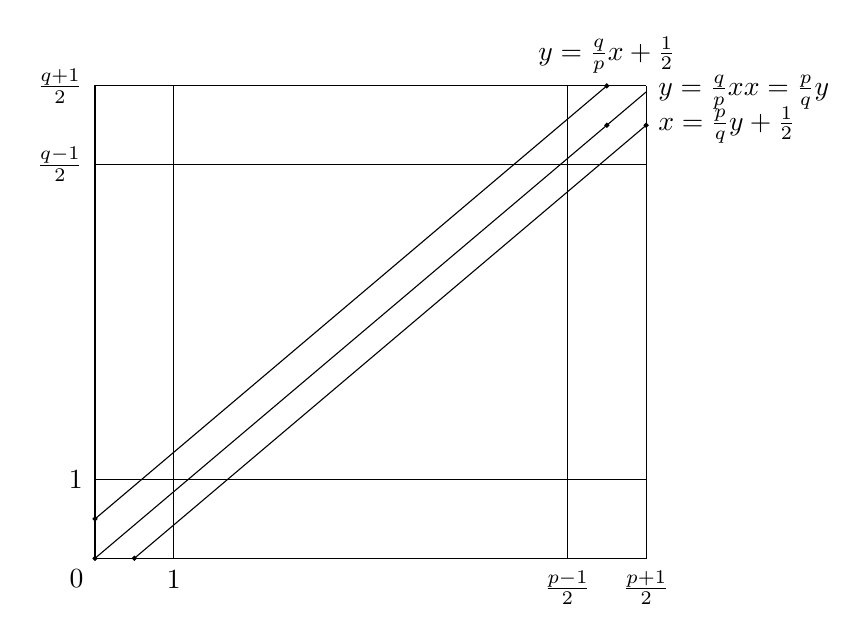
\begin{tikzpicture}
\draw(0,0)to(7,0)to(7,6);
\draw(0,0)to(0,6)to(7,6);
%\draw(0,0)to(13/2,11/2);
\draw(0,0)to(7,7*11/13);
\draw(1,0)to(1,6);
\draw(6,0)to(6,6);
\draw(0,1)to(7,1);
\draw(0,5)to(7,5);
\draw(0,1/2)to(13/2,6);
\draw(1/2,0)to(7,11/2);
\node[circle,draw,fill,color=black,inner sep=0.5pt,label=below left:$0$]at(0,0){};
\node[circle,inner sep=0.5pt,label=below:$1$]at(1,0){};
\node[circle,inner sep=0.5pt,label=left:$1$]at(0,1){};
\node[circle,inner sep=0.5pt,label=below:$\frac{p-1}{2}$]at(6,0){};
\node[circle,inner sep=0.5pt,label=below:$\frac{p+1}{2}$]at(7,0){};
\node[circle,inner sep=0.5pt,label=left:$\frac{q-1}{2}$]at(0,5){};
\node[circle,inner sep=0.5pt,label=left:$\frac{q+1}{2}$]at(0,6){};
\node[circle,draw,fill,color=black,inner sep=0.5pt]at(0,1/2){};
\node[circle,draw,fill,color=black,inner sep=0.5pt]at(1/2,0){};
\node[circle,draw,fill,color=black,inner sep=0.5pt]at(13/2,11/2){};
\node[circle,draw,fill,inner sep=0.5pt,label=above:{$y=\frac{q}{p}x+\frac{1}{2}$}]at(13/2,6){};
\node[circle,draw,fill,inner sep=0.5pt,label=right:{$x=\frac{p}{q}y+\frac{1}{2}$}]at(7,11/2){};
\node[circle,inner sep=0.5pt,label=right:{$y=\frac{q}{p}x\co x=\frac{p}{q}y$}]at(7,7*11/13){};
\end{tikzpicture} \]
